\chapter{Teoretický rámec}\label{chapter:teorie}

V této kapitole představíme potřebné teoretické koncepty, které bude využívat výsledná aplikace.
Mezi tyto koncepty patří \acrfull{er} model a nově vyvíjený konceptuální model v podobě schematické kategorie~\cite{svoboda_categorical_2021} v rozšířené verzi navržené vedoucím práce.

\section{\acrlong{er}}\label{section:entity-relationship}

Datový model \acrfull{er} poprvé představil Peter Pin-Shan Chen už v roce 1976~\cite{chen_er_1976}.
Od té doby se však \acrshort{er} vyvíjel, jak se potřeby datového modelování rozšiřovaly.
\acrshort{er} není standardizováno, ale jednu moderní verzi představili Atzeni, Ceri, Paraboschi a Torlone~\cite[s.~163-179]{atzeni_database_1999}.
Na jejich \acrshort{er} modelu založíme ten náš, který zde popíšeme.

V Tabulce~\ref{tab:er-constructs} jsou vyobrazeny jednotlivé konstrukty \acrshort{er} modelu.

\begin{table}[htb]
  \centering
  \begin{tabular}{@{}rm{9cm}@{}} \toprule
    Konstrukt             & Vizuální reprezentace                                     \\ \midrule
    Entitní typ           & {\centering
\includegraphics{../img/er-model/entity.pdf}}  \\
    Vztahový typ          & 
\includegraphics{../img/er-model/relationship.pdf}        \\
    Atribut               & 
\includegraphics{../img/er-model/attribute.pdf}           \\
    Složený atribut       & 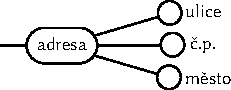
\includegraphics{../img/er-model/composite-attribute.pdf} \\
    Interní identifikátor & 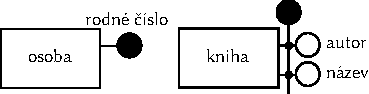
\includegraphics{../img/er-model/identifier.pdf}          \\
    Externí identifikátor & 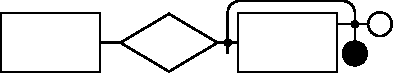
\includegraphics{../img/er-model/external-identifier.pdf} \\
    Zobecnění             & 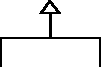
\includegraphics{../img/er-model/generalization.pdf}      \\ \bottomrule
  \end{tabular}
  \caption[Grafická reprezentace konstruktů \acrshort{er} modelu]{Grafická reprezentace konstruktů \acrshort{er} modelu, upraveno a přeloženo~\cite[s.~164, Obr.~5.4]{atzeni_database_1999}}
  \label{tab:er-constructs}
\end{table}

Zde blíže popíšeme jejich sémantiku:
\begin{itemize}
  \item Entitní typ (Entity Type) reprezentuje předpis pro instance entit reálného světa.
        Každý entitní typ má jméno, které je unikátní v daném schématu.
  \item Vztahový typ (Relationship Type) reprezentuje vztah mezi dvěma nebo více (ne nutně různými) entitními typy.
        Každý vztahový typ má jméno.
  \item Atribut (Attribute) reprezentuje vlastnost entitních nebo vztahových typů.
        Každý atribut má jednoznačné jméno.
  \item Složený atribut (Composite Attribute) je atribut, který má sám atributy.
        Zakazujeme však další větvení, tedy atributy složeného atributu už samy nemohou být složené.
        Každý složený atribut má sám jméno, podobně jako jeho vlastní atributy.
  \item \label{def:cardinality}Kardinalita (Cardinality) je dvojice $(a, b) \in \set{\zero, \one}\times \set{\one, \many}$, kde $a$ nazýváme minimální kardinalita (spodní hranice) a $b$ maximální kardinalita (horní hranice).
        Kardinalitu musí mít každý atribut a každý účastník vztahového typu.
        Výchozí kardinalita je \oneone{} a ve schématu se většinou neuvádí.
        Spodní hranice 0 znamená, že účast je volitelná; hranice 1 znamená, že účast je povinná.
        Horní hranice 1 znamená, že účast je nejvýše jedna; hranice~\many{} znamená, že účastí je libovolný počet.
        \begin{itemize}
          \item Hranice kardinalit pro jednotlivé účastníky vztahových typů vyjadřují minimální a resp. maximální počet výskytů jednotlivých instancí účastníků v tomto vztahu.
          \item Hranice kardinalit u atributů vyjadřují minimální a resp. maximální počet hodnot atributu, které se vztahují k dané instanci entity/vztahu.
        \end{itemize}
  \item Identifikátor (Identifier) umožňuje jednoznačně rozlišit (identifikovat) instance entitních typů.
        Pro každý entitní typ je povinný alespoň jeden identifikátor, ale může jich být více.
        Každý identifikátor je tvořen buď
        \begin{itemize}
          \item jedním nebo více atributy daného entitního typu; takový identifikátor nazýváme \emph{interní}, nebo
          \item jedním, nebo více vztahovými typy, jichž se daný entitní typ účastní, a žádným či libovolným množstvím atributů daného entitního typu; takový identifikátor nazýváme \emph{externí}.
        \end{itemize}
  \item Zobecnění (generalization), nebo také ISA hierarchie\footnote{ISA z anglického \enquote{is a}, analogicky ke vztahu \enquote{has a}} (ISA Hierarchy), vyjadřuje vztah podobný dědičnosti v objektově orientovaném programování.
        Jde o vztah mezi entiním typem $E$ zvaným \emph{rodič} a jedním nebo více \emph{dětmi} $E_1, \dots, E_n$.
        Všechny vlastnosti rodiče (atributy, identifikátory, spojené vztahové typy a další ISA hierarchie) jsou i vlastnosti každého z dětí.
        Každá instance dítěte je také instancí rodiče.
\end{itemize}

Entitní typy, které nemají ani jeden interní identifikátor (musí mít tedy externí), nazýváme \emph{slabé} entitní typy (weak entity types).
Pokud mají interní identifikátor, nazýváme je \emph{silné} entitní typy (strong entity types).

Vztahový typ se externí identifikace může účastnit nejvýše od jednoho účastníka.
Jinak řečeno, pokud je vztahový typ součástí slabého identifikátoru nějakého entitního typu, daný vztahový typ už nemůže být součástí slabého identifkátoru jiného entitního typu.
Jeden entitní typ však může mít více externích identifikátorů, který každý zahrnuje daný vztahový typ.
Nicméně, externí identifikace se může řetězit, jako na Obrázku~\ref{fig:er-external-identifier-chain}.
Nesmí ovšem vzniknout orientovaný cyklus, a to ani v kombinaci s ISA hierarchiemi.
Formálněji -- pokud vytvoříme orientovaný graf $G=(V,E)$ takový, že
\begin{itemize}
  \item vrcholy $V$ jsou entitní typy a
  \item hrany $E$ jsou
        \begin{itemize}
          \item pro každý externí identifikátor od identifikovaného entitního typu $a$ k identifikujícímu entitnímu typu $b$ orientovaná hrana $(a, b)$,
          \item pro každou ISA hierarchii pro každý vztah rodič-dítě, kde $a$ je dítě a $b$ je rodič, orientovaná hranu $(a, b)$,
        \end{itemize}
\end{itemize}
pak graf $G$ musí být acyklický.

V \acrshort{er} se nesmí vyskytovat identifikátory, které jsou redundantní.
Pro každé dva identifikátory jednoho entitního typu $I, J$, pokud $J\subset I$, pak $I$ je \emph{redundantní}, protože k identifikaci entitního typu stačí $J$.
Všechny atributy a vztahové typy v $I\setminus J$ nejsou potřeba k identifikaci.
Ukázka redundantního identifikátoru je na Obrázku~\ref{fig:redundant-ids}.

\begin{figure}[!htb]
  \centering
  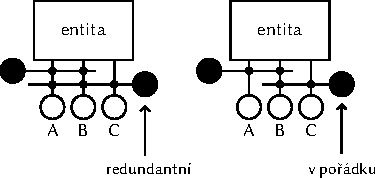
\includegraphics[width=\maxwidth{\textwidth}]{../img/er-model/redundant-ids.pdf}
  \caption{Ukázka redundantního a neredundantního identifikátoru}
  \label{fig:redundant-ids}
\end{figure}

Entitní typ, který má externí identifikátor, musí být účastněn vztahového typu (jímž je identifikován) s kardinalitou $(\one, \one)$.
Teoreticky by se mohl účsatnit i jinou kardinalitou, ale pro naše účely tyto situace modelovat nebudeme.

\begin{figure}[!htb]
  \centering
  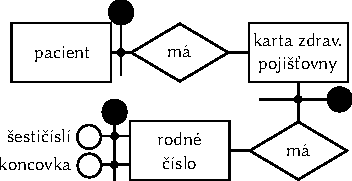
\includegraphics[width=\maxwidth{\textwidth}]{../img/er-model/external-id-chain.pdf}
  \caption{Zřetězení externích identifikátorů}
  \label{fig:er-external-identifier-chain}
\end{figure}

U kardinality poznamenejme, že se v \acrshort{er} modelu často dovoluje použít jako hranice libovolná nezáporná celá čísla, tedy $(a, b)\in \mathbb N_0\times \left(\mathbb N_0 \cup \set{\many}\right)$, tž.~$a\leq b$ (dodefinujeme $\forall a\in\mathbb N_0\colon a < \many$).
Dají se tak vyjádřit přesnější omezení, např. že jeden uživatel může mít maximálně 5 bankovních účtů.
Ovšem námi definované hranice kardinality vyjadřují volitelnost/povinnost pro spodní hranici a jednočetnost/mnohočetnost pro horní hranici.
Pokryjeme jimi z teoretického pohledu a s ohledem na povahu konstruktů v nejrůznějších logických modelech všechny strukturálně odlišné situace, které by mohly nastat.

Dále upozorněme, že místo~\many{} se v \acrshort{er} modelu může použít symbol \texttt{n} nebo \texttt{N} pro vyjádření \enquote{libovolného počtu}.
Důležitá je ale konzistentnost, aby se v jednom modelu nevyskytovaly dva různé symboly, což by mohlo zmást čtenáře.
V této práci budeme používat pouze symbol~\many{}.

\section{Schematická kategorie}\label{section:schemcat}

V této sekci popíšeme mechanismus pro konceptuální modelování s názvem schematická kategorie společně s teorií kategorií, na které je založena.
Nejdříve ale představíme motivaci za uvedením nového způsobu konceptuálního modelování.

\subsection{Motivace}

Při začátku vývoje databázových systémů bylo popsáno několik databázových modelů dat.
Už v roce 1975 je ANSI rozdělila do tří vrstev~\cite{steeljr._interimreport_1975}.
\begin{itemize}
  \item Konceptuální vrstva popisuje část světa, na kterou vymezujeme svůj diskurz.
  \item Logická vrstva popisuje logickou strukturu dat (např. graf, tabulka, \dots).
  \item Fyzická vrstva popisuje, jak jsou data fyzicky uložena.
\end{itemize}

Přestože databázových modelů bylo navrženo několik, časem se ukázalo, že nejužitečnější je ten relační.
To proto, že data byla často tabulkové povahy.
Pokud výjimečně nebyla takové povahy, musela se relačnímu modelu přizpůsobit.

S příchodem potřeby zpracování velkých dat (Big Data)~\cite{cron_bigdata_2012} se ukázalo, že relační model není dostačující.
Ve velkém množství dat, která spolu nutně nesouvisí, není totiž vždy vhodné hledat tabulkovou strukturu.
Ukazuje se, že většina dat reálného světa není relačního charakteru.
V různých situacích jsou tedy vhodné různé databázové systémy s různými logickými modely.
Namísto přizpůsobování dat logickému modelu se postupně začal více přizpůsobovat logický model datům.
Dokonce se začalo používat více databázových systémů najednou v rámci jednoho informačního systému.
Například pro cache lze použít key/value store, pro data různorodé povahy lze použít dokumentové databáze a pro silně strukturovaná data starší relační databáze.

Naše vize do budoucna je mít jediný databázový systém, který má jediné rozhraní, jediný způsob modelování dat a jediný dotazovací jazyk, ale zároveň není závislý na fyzické vrstvě.
V současných systémech je často tvorba a iterace databázových schémat časově náročná a obtěžující.
Chceme proto sloučit konceptuální a logickou vrstvu a předejít tak problémům a lidskému rozhodování při převodu mezi nimi.
Vznikne tak pouze jedna vrstva, ve které se pracuje unifikovaným, konceptuálním způsobem.

Prvním krokem v této vizi by mohly být schematické kategorie, které uživateli umožní popsat strukturu dat, se kterými chce v databázi pracovat.
Jejich koncept popisují Martin Svoboda, Pavel Čontoš a Irena Holubová~\cite{svoboda_categorical_2021}.

Prostředky \acrshort{er} jsou vhodné ke konceptuálnímu modelování, nicméně mají několik nevýhod.
Některé z nich zde identifikujeme.
\begin{itemize}
  \item V \acrshort{er} lze často modelovat jeden případ mnoha způsoby a není předem jasné, který z nich je nejlepší.
        Schematické kategorie většinu takových rozdílů smažou, zejména rozdíly mezi entitními typy, vztahovými typy a atributy.
        Často totiž tyto rozdíly nejsou důležité.
  \item \acrshort{er} zavádí několik omezení, např.~vztahové typy nemohou mít interní identifikátor a složené atributy se nemohou libovolně větvit.
        Tato omezení vznikají, protože se historicky \acrshort{er} používalo zejména pro konceptuální modelování pro relační databáze.
        Libovolně větvené atributy se těžko převedou do relačního modelu.
\end{itemize}

\acrfull{uml}~\cite{omg_uml_2017} také umožňuje vytvářet konceptuální schémata.
Při vývoji software, zvlášť při práci v týmech, je většinou zvoleno \acrshort{uml} oproti \acrshort{er}.
Je to dáno existencí rozličných nástrojů na vytváření \acrshort{uml} diagramů a nástrojů na automatizaci převodu do logické vrstvy.
Vyjadřovací schopnost \acrshort{uml} je nicméně menší, než u \acrshort{er}.
Postupným vývojem \acrshort{uml} se expresivnost dodává.
Nicméně dosahuje se toho přes konstrukty (např.~stereotypy), u kterých lze poznat, že nesouhlasí s původní myšlenkou \acrshort{uml}.

\subsection{Teorie kategorií}

Nejdříve popíšeme obecný pojem kategorie z teorie kategorií, na níž je schematická kategorie založena.

Kategorie je matematická struktura, která zobecňuje mnoho jiných matematických struktur.
Umožňuje tak mimo jiné studovat vztahy mezi nimi.
Poprvé byla představena Eilenbergem a MacLanem v roce 1945~\cite{eilenberg_generaltheory_1945}.

Kategorie $C=(\mathcal O, \mathcal M, \circ)$ se skládá
z \begin{itemize}
  \item množiny objektů $\mathcal O$,
  \item množiny morfismů $\mathcal M$; každý morfismus $f \in \mathcal M$ má zdrojový objekt $A\in\mathcal O$ (budeme naývat také \emph{doména}), cílový objekt $B\in\mathcal O$ (také \emph{kodoména}), ne nutně různý, a zapisujeme $f: A\to B$ ($f$ je morfismus z $A$ do $B$),
  \item operace skládání $\circ\colon \mathcal M\times\mathcal M \to \mathcal M$; pro každé dva morfismy $f,g\in\mathcal M$, tž. $f\colon A\to B, g\colon B\to C$, musí $g\circ f\in \mathcal M$ (tranzitivita); pro tuto operaci navíc platí vlastnosti
        \begin{itemize}
          \item asociativita -- pro morfismy $f,g,h\in\mathcal M$ takové, že $f\colon A\to B, g\colon B\to C, h\colon C\to D$, platí $h\circ (g \circ f) = (h\circ g)\circ f$,
          \item identitní morfismy -- pro každý morfismus $f\in\mathcal M, f\colon A\to B$ a jeho objekty $A$, resp. $B\in\mathcal O$ existují morfismy $1_A$, resp. $1_B\in\mathcal M$, tž. $f\circ 1_A = f = 1_B\circ f$; morfismy $1_A$, resp. $1_B$ nazýváme \emph{identitní morfismy}.
        \end{itemize}
\end{itemize}

Objekty a morfismy lze definovat i obecněji s použitím tříd místo množin, ale pro naše účely budou stačit množiny.

Jako jednoduchý příklad kategorie uvedeme reálná čísla s neostrou nerovností.
Objekty této kategorie jsou reálná čísla $\mathcal O=\R$.
Pro každá reálná čísla $A,B\in\R$ přidáme morfismus $f\colon A\to B$ právě tehdy, když $A\leq B$.
Pro všechny morfismy $f,g\in\mathcal M$ a objekty $A, B, C\in\mathcal O$ takové, že $f\colon A\to B$ a $g\colon B\to C$ definujme $g\circ f=h$, kde $h\colon A\to C$ a $h\in\mathcal M$.

Kategorie je možné vizuálně reprezentovat orientovaným multigrafem, kde vrcholy jsou objekty a orientované hrany morfismy.
Příklad této vizualizace je na Obrázku~\ref{fig:category-example}.
Jedná se o kategorii se třemi objekty $A, B, C$.
Všimněme si, že každý objekt má svůj identitní morfismus.

\begin{figure}[!htb]
  \shorthandoff{"}
  \centering
  % https://tikzcd.yichuanshen.de/#N4Igdg9gJgpgziAXAbVABwnAlgFyxMJZABgBpiBdUkANwEMAbAVxiRAEEQBfU9TXfIRQBGclVqMWbAELdeIDNjwEio4ePrNWiEAGFu4mFADm8IqABmAJwgBbJGRA4ISURK1sLcyzfuI3zkgATNSaUjrG3iDWdg7UgYgh7uEgxgA6aQDGWFaZAARe1Ax0AEYwDAAK-MpCIFZYxgAWOFExfo4JjgwQEGhEQQDsZBaMcDDixWWV1YJs9U0toZLaIMIA+pw8PrH+8S67IN29RACcw6PjRaXlVUqzOvPNIEseOuuyW9G+wXs-hz19FBnUgjBhjCbXaZ3FQPBpPF4pdb6LgULhAA
  \begin{tikzcd}
    A \arrow[r, "f"] \arrow[rd, "g\circ f"'] \arrow["1_A"', loop, distance=2em, in=215, out=145] & B \arrow[d, "g"] \arrow["1_B"', loop, distance=2em, in=35, out=325] \\
    & C \arrow["1_C"', loop, distance=2em, in=35, out=325]
  \end{tikzcd}
  \caption{Příklad kategorie}%
  \label{fig:category-example}%
  \shorthandon{"}
\end{figure}

\subsection{Schematická kategorie}

Schematická kategorie je mechanismus na popis konceptuálního schématu dat založený na teorii kategorií.
Oproti~\acrshort{er} má schematická kategorie větší vyjadřovací sílu.
Její koncept společně s algoritmem převodu z \acrshort{er} schématu do schematické kategorie uvádí~\cite{svoboda_categorical_2021}.
My však použijeme upravenou definici schematické kategorie navrženou vedoucím práce.

Nejprve zavedeme pomocný pojem \emph{signatura}.
Jedá se o řetězec nad abecedou symbolů $\N$.
Prázdný řetězec značíme $\varepsilon$.
Operaci zřetězení značíme symbolem $\cdot$ tečky.
Příklady signatur: $\varepsilon$, $13$, $13\cdot 7$.

Formálně je schematická kategorie instance kategorie $(\mathcal O, \mathcal M, \circ)$ taková, že
\begin{itemize}
  \item každý objekt této kategorie má strukturu trojice: (identita, název, množina identifikátorů), kde
        \begin{itemize}
          \item identita je libovolný symbol z $\N$, který umožňuje rozlišit a unikátně identifikovat každý objekt; tedy speciálně i pro případ, kdy by všechny ostatní složky měl totožné s jiným objektem,
          \item název reprezentuje textovým řetězcem uživatelské jméno daného objektu, může být i prázdný, pak ho značíme $\bot$,
          \item množina identifikátorů obsahuje identifikátory; každý jednotlivý identifikátor je množina identit a vyjadřuje, čím lze daný objekt konceptuálně identifikovat (podobně jako identifikátory z \acrshort{er}),
        \end{itemize}
  \item každý morfismus má strukturu osmice: (signatura, doména, kodoména, název, kardinalita, duplicity, uspořádání),
        \begin{itemize}
          \item signatura byla již popsána jako pomocný pojem; její účel je umožnit (společně s doménou a kodoménou) rozlišit a unikátně identifikovat každý morfismus v daném schématu; jedná se o řetězec vyjadřující orientovanou cestu, složený ze signatur bázových morfismů (zřetězujeme ve stejném pořadí jako se zapisuje skládání morfismů v kategorii, viz Obrázek~\ref{fig:morphism-signatures}),
          \item doména a kodoména odpovídají zdrojovému a cílovému objektu tohoto morfismu,
          \item směr je buď \zero{} (tam) nebo \one{} (zpět) s výchozí hodnotou \zero{}; hodnota \one{} vyjadřuje, že tento morfismus je pouze inverze k jinému, dodaná pro úplnost modelu,
          \item název je uživatelské jméno tohoto morfismu, může být i prázdné $\bot$,
          \item kardinalita je dvojice (min, max), která odpovídá kardinalitě z \acrshort{er} v Sekci~\ref{def:cardinality},
          \item duplicity a uspořádání jsou booleovské hodnoty (\texttt{true}/\texttt{false}), které konceptuálně modelují, zda jsou pro vztažené instance (modelovány kodoménou), která jsou morfismem spojena k vztahované instanci (modelována doménou), povoleny duplicity, resp. jestli mají být uspořádány; tyto hodnoty mají význam, pouze pokud je horní hranice kardinality tohoto morfismu \many; výchozí hodnota obou složek je proto \texttt{false}.
        \end{itemize}
\end{itemize}

Morfismy schematické kategorie rozdělíme na několik vzájemně disjunktních druhů.
Příklad každého druhu lze pozorovat na Obrázku~\ref{fig:morphism-signatures}.
\begin{itemize}
  \item \emph{Bázové} (base) morfismy jsou ty, které vyjadřují konceptuální spojení dvou objektů ze schématu (tedy odpovídají jednotlivým spojením z ER); jejich signatura je jeden unikátní symbol z abecedy.
  \item \emph{Identitní} (identity) morfismy jsou ty, které vznikly jen kvůli splnění stejnojmenného axiomu z definice kategorie; jejich signatura je $\varepsilon$.
  \item \emph{Odvozené} (derived) morfismy jsou ty, které vznikly kvůli tranzitivitě (tedy aby byly morfismy uzavřené na operaci skládání); jejich signatura je opravdová cesta -- zřetězené signatury morfismů, ze kterých byl tento morfismus vytvořen.
\end{itemize}

Ve schematické kategorii bez újmy na vyjadřovací schopnosti zakážeme bázové smyčky (tj. bázový morfismus, jehož doména a kodoména je totožná).
Pokud chceme vyjádřit rekurzivní vztah, můžeme bázovou smyčku nahradit objektem, který tento vztah reprezentuje.
Navíc dodáme dva bázové morfismy, které spojí objekt vztahu s objektem, jehož se vztah týká.

Operaci skládání morfismů $\circ$ ve schematické kategorii lze definovat následovně.
Pro dva morfismy $f,g\in\mathcal M$ a objekty $A,B,C\in \mathcal O$ takové, že $f\colon A\to B, g\colon B\to C$ a
\begin{itemize}
  \item $f$ se skládá z $(\sig_1, \dom_1, \mathit{mid}, \name_1, (\minn_1, \maxx_1), \dup_1, \ord_1)$,
  \item $g$ se skládá z $(\sig_2, \mathit{mid}, \cod_2, \name_2, (\minn_2, \maxx_2), \dup_2, \ord_2)$,
\end{itemize}
je jejich složením $g\circ f$ morfismus $h\in M, h\colon A\to C$ skládající se z
\begin{multline*}
  (\sig_2\cdot \sig_1, \dom_1, \cod_2, \bot, (\min(\minn_1, \minn_2), \max(\maxx_1, \maxx_2)),\\
  \dup_1 \lor \dup_2, \ord_1\land \ord_2)\,.
\end{multline*}

Protože $f$ a $g$ na sebe navazují, musí být kodoména $f$ totožná s doménou $g$, označili jsme ji $\mathit{mid}$.
Dále, protože $dom_1, \mathit{mid}$ a $cod_2$ odpovídají identitám objektů $A, B, $ resp. $C$, složený morfismus má doménu $dom_1$ a kodoménu $cod_2$.
Když u jednoho z morfismů záleží na duplicitách bude záležet i u složeného na duplicitách.
Aby záleželo u složeného morfismu na uspořádání, musí však záležet na uspořádání u obou skládaných morfismů.

\begin{figure}[!htb]
  \centering
  \begin{tikzpicture}
    \tikzset{vertex/.style={shape=circle,draw,minimum size=1em}}
    \tikzset{edge/.style = {->,> = latex'}}
    \node[vertex] (a) {};
    \node[vertex] (b) [right=of a] {};
    \node[vertex] (c) [right=of b] {};

    \draw[edge] (a) to[bend left] node[above] {$13$} (b) ;
    \draw[edge] (b) to[bend left] node[above] {$7$}  (c);
    \draw[edge] (a) to[bend right] node[below] {$7\cdot 13$} (c);
    \draw[edge] (a) to[loop left] node[left] {$\varepsilon$} (a);
    \draw[edge] (b) to[loop above] node[above] {$\varepsilon$} (b);
    \draw[edge] (c) to[loop right] node[right] {$\varepsilon$} (c);
  \end{tikzpicture}
  \caption{Signatury morfismů, $\cdot$ je operace konkatenace (zřetězování) symbolů}
  \label{fig:morphism-signatures}
\end{figure}

\begin{figure}[!htb]
  \centering
  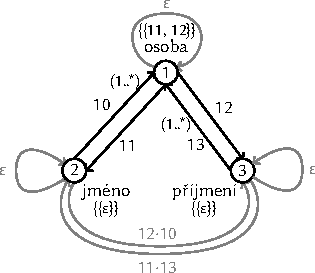
\includegraphics[width=\maxwidth{\textwidth}]{../img/schemcat-diagrams/raw-schemcat-example.pdf}
  \caption{Příklad schematické kategorie}
  \label{fig:raw-schemcat}
\end{figure}

Na Obrázku~\ref{fig:raw-schemcat} je příklad schematické kategorie se třemi objekty.
Objekt \enquote{osoba} je identifikován dohromady dvojicí objektů \enquote{jméno} a \enquote{příjmení}.
Objekty \enquote{jméno} a \enquote{příjmení} jsou každý identifikován sám sebou, proto jim náleží jediný identifikátor vždy v podobě $\set{\varepsilon}$.
Na obrázku jsou dále bázové morfismy (plné čáry) se svými signaturami a kardinalitami, přičemž výchozí (\one{}, \one{}) neuvádíme.
Identitní a dva vybrané odvozené morfismy jsou vyznačeny čárkovanými křivkami.
Jejich signatury jsou složené řetězce, resp. prázdné řetězce $\varepsilon$.

\section{Vizualizace schematické kategorie}\label{section:vsk}

Schematická kategorie je formálně zadefinovaný model.
Pro potenciálního uživatele schematické kategorie je její jednolitost a informativnost příliš nepřehledná.
Navrhněme proto způsob vizualizace, který přinese odlišení a zvýraznění některých důležitých konstruktů, včetně vyobrazení některých složek objektů a morfismů, ale zachovává vyjadřovací sílu představených schematických kategorií.
Pojmenujme ho \acrfull{vsk}.

Objekt schematické kategorie, který má jediný identifikátor $\set{\varepsilon}$ nazveme \emph{self-identifikovaný} objekt.
Instance takových objektů jsou identifikovány svými hodnotami.
Jsou tedy podobné atributům z \acrshort{er}, a proto je budeme značit kružnicí.

Objekty, které nejsou self-identifikované, jsou určitě identifikované jinými objekty.
Jsou významově analogické entitním nebo vztahovým typům z \acrshort{er}.
Značit je budeme obdélníkem.

Dvojice duálních morfismů budeme vždy značit jedinou neorientovanou hranou vedoucí mezi příslušnými objekty.
Nebudeme vizualizovat identitní ani odvozené morfismy.
Neukážeme ani signatury morfismů, nejsou totiž potřeba.

Kardinality morfismů budeme vykreslovat blízko domény patřičného morfismu.
Výchozí kardinality zobrazovat nebudeme.

Identifikátory objektů budeme značit stejně jako v \acrshort{er} přeškrtnutím patřičných morfismů, a i v případě jednoduchých identifikátorů.

Složky morfismu \emph{uspořádání} a \emph{duplicity} budou pro výchozí hodnoty (\texttt{false} a \texttt{false}) neviditelné.
Jinak v cílovém objektu na konci spojovací čáry morfismu vyznačíme hodnotu \texttt{true} uspořádání symbolem $\leq$, resp. $+$ pro duplicity.

Uživatelské názvy objektů i morfismů budeme vykreslovat, podobně jako v \acrshort{er}, u self-identifikovaných objektů v blízkosti objektu, jinak uvnitř obdélníku.

Na Obrázku~\ref{fig:schemcat-visualization-example} vidíme diagram odpovídající schematické kategorii z Obrázku~\ref{fig:raw-schemcat}.
Sémantika kardinalit (\one, \many) u obou obrázků taková, že konceptuálně může jedno jméno, resp. příjmení patřit více osobám.

\begin{figure}[!htb]
  \centering
  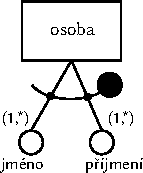
\includegraphics[width=\maxwidth{\textwidth}]{../img/schemcat-diagrams/schemcat-visualization-example.pdf}
  \caption{Příklad vizualizace schematické kategorie}
  \label{fig:schemcat-visualization-example}
\end{figure}

Na Obrázku~\ref{fig:scv-ord-dup} lze vidět vizualizaci schematické kategorie, která má u jednoho z morfismů aktivní uspořádání a duplicity.
Význam tohoto schématu je takový, že seznam úkolů může mít libovolný počet úkolů, a to dokonce se stejným popisem (duplicity) a že je důležité udržovat informaci o pořadí, ve kterém byly jednotlivé úkoly přidávány (uspořádání).

\begin{figure}[!htb]
  \centering
  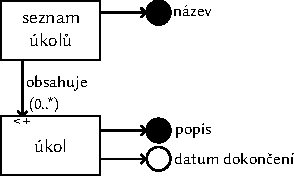
\includegraphics[width=\maxwidth{\textwidth}]{../img/schemcat-diagrams/scv-ord-dup.pdf}
  \caption{Vizualizace schematické kategorie s využitými složkami \emph{uspořádání} a \emph{duplicity}}
  \label{fig:scv-ord-dup}
\end{figure}

\section{Převod ER na schematickou kategorii}

Algoritmus převodu z \acrshort{er} na schematickou kategorii už popsali Svoboda a kol.~\cite[s.~192-196]{svoboda_categorical_2021}.
Pro naši upravenou verzi schematické kategorie však musíme upravit i algoritmus převodu.

Uvědomme si nejdříve, že v \acrshort{er} diagramu, který dostaneme nemusí mít některý entitní typ ani jeden vlastní atribut.
Přestože každý entitní typ musí mít alespoň jeden identifikátor, tento identifikátor nemusí být tvořen vlastním atributem.
To ze dvou důvodů, které se vzájemně nevylučují:
\begin{enumerate}
  \item entitní typ může být dítě v hierarchii, kdy dědí identifikátor od rodiče,
  \item nebo se může jednat o slabý entitní typ, který má pouze externí identifikátory, které neobsahují ani jeden interní identifikátor.
\end{enumerate}

Kvůli definici schematické kategorie budeme vybírat unikátní identifikátory z abecedy $\N$.
V $\N$ je k tomu určitě dostatek symbolů.

Mějme tedy validní \acrshort{er} diagram.
Převedeme ho na schematickou kategorii.

Nejdříve definujeme správné pořadí, ve kterém převádět entitní typy.
Vezměme závislostní graf, který jsme definovali kvůli zakázání cyklů v Sekci~\ref{section:entity-relationship}.
Tento graf je z definice orientovaný a pro korektní \acrshort{er} je acyklický.
Jedná se tedy o \acrshort{dag}.
Vezměme jeho libovolné topologické uspořádání.
Entitní typy budeme převádět od \emph{největšího} prvku tohoto uspořádání k nejmenšímu.
To proto, abychom vždy nejdříve převedli nějaký takový entitní typ, pro který už jsou vyřešené ty, na kterých je identifikačně závislý.
Jinak by náš převod slabého entitního typu nemusel mít korektní identifikátory.
S tímto pořadím budeme počítat po celý algoritmus.

Kvůli délce algoritmu zde nejdříve naznačíme hrubý postup, než popíšeme jednotlivé kroky.
Začneme s prázdnou schematickou kategorií a postupně budeme převádět konstrukty \acrshort{er} do konstruktů schematické kategorie:
\begin{itemize}
  \item Nejdříve vytvoříme objekt každý jednoduchý nebo složený atribut a spojíme je morfismy (složené atributy s jejich atributy).
  \item Následně vytvoříme objekt pro každý entitní typ, ale ještě mu nepřevedeme identifikátory, protože nemáme v tuto chvíli všechny potřebné morfismy.
  \item Proto se následně budeme věnovat vztahovým typům -- vytvoříme pro každý z nich objekt (zatím zase bez identifikátorů) a spojíme ho morfismy s jeho atributy a účastnícími se entiními typy.
  \item Poté se budeme věnovat identifikátorům objektů entitních typů a vztahových typů.
  \item Nakonec převedeme ISA hierarchie, včetně zděděných identifikátorů.
\end{itemize}

Pro každý (jednoduchý nebo složený) atribut z \acrshort{er} vytvořme odpovídající objekt schematické kategorie (s odpovídajícím názvem a unikátní identitou).
Množina identifikátorů objektu bude vždy obsahovat pouze jediný identifikátor $\set{\varepsilon}$, půjde tedy o self-identifikovaný objekt.

Pro každý složený atribut $C$ z \acrshort{er} diagramu a pro každý jeho atribut $A$ zvolíme unikátní symbol $n\in N$ a vytvoříme dva duální bázové morfismy mezi odpovídajícími objekty $O_C$ a $O_A$.
\begin{align*}
  (n, \mathit{identita}\ O_C, \mathit{identita}\ O_A, \bot, \oneone, \false, \false)\,, \\
  (n, \mathit{identita}\ O_C, \mathit{identita}\ O_A, \bot, \onemany, \false, \false)\,.
\end{align*}\mcomment{Mají doména/kodoména duálních morfismů být ve stejném pořadí? Nemám prohodit u toho druhého doménu s kodoménou?}
Signatury těchto morfismů jsou stejné, abychom poznali, že jsou k sobě duální.
Příčí se to sice unikátnosti, kterou jsme při definicích vyžadovali, ale prakticky je tento přístup vhodný.

Pro každý entitní typ $E$ z \acrshort{er} diagramu vytvoříme jemu odpovídající objekt $O_E$, ale zatím necháme množinu identifikátorů prázdnou.
Pro atributy $E$ vezmeme každý odpovídající objekt $O_A$ a vytvoříme bázový morfismus mezi $O_E$ a $O_A$ (i k němu duální) podobně jako výše.
Kardinalitu směrem k atributu nastavíme na kardinalitu $A$ vzhledem k $E$ a kardinalitu směrem zpět na
\begin{itemize}
  \item \oneone{} pokud je $A$ jednoduchý identifikátor $E$,
  \item \onemany{} pokud je $A$ součástí složeného identifikátoru $E$,
  \item jinak \zeromany{} u obyčejného atributu.
\end{itemize}

Pro každý vztahový typ $R$ z \acrshort{er} diagramu vytvoříme odpovídající objekt $O_R$ a necháme množinu identifikátorů prázdnou.
Všechny atributy a složené atributy $R$ spojíme s $O_R$ stejně jako tomu bylo u entitních typů a jejich atributů.
Mezi $R$ a každým účastníkem tohoto vztahového typu, označme $E$, (resp. mezi jejich odpovídajícími objekty) vytvoříme bázový morfismus s kardinalitou tam stejnou jako je kardinalita $E$ vzhledem k $R$.
Kardinalita směrem zpět (tedy kardinalita duálního morfismu) bude stejná jako kardinalita $R$ vzhledem k $E$.

Nyní se můžeme věnovat identifikátorům entitních typů.
Ty převádíme také v pořadí, které jsme pro entitní typy určili.
Pro každý identifikátor $I$ entitního typu $E$ tedy vytvoříme nový identifikátor pro odpovídající objekt schematické kategorie $O_E$.
Převod každého prvku identifikátoru $I$ proběhne následovně.
\begin{itemize}
  \item Pokud se jedná o vlastní atribut $E$, převedeme ho jednoduše na signaturu morfismu, který spojuje $O_E$ s odpovídajícím objektem daného atributu.
  \item Pokud se jedná o vztahový typ, najdeme orientovanou cestu přes odpovídající morfismy z $E$ do každého $E_i$ entitního typu, do kterého vede externí identifikátor.
        Nechť $c$ je zřetězení signatur morfismů, přes které tato cesta vede.
        Dále, nechť $O_i$ je objekt odpovídající $E_i$.
        Pro každý identifikátor $I_k$ z množiny identifikátorů objektu $O_i$ vytvoříme $S\coloneqq \set{c_k\cdot c\mid c_k\in I_k}$.
\end{itemize}
Sjednocením všech těchto množin $S$ a množiny signatur odpovídajících vlastním atributům získáme množinu signatur, která tvoří jeden identifikátor objektu $O_E$, který odpovídá \acrshort{er} identifikátoru $I$.
Zřetězili jsme totiž signatury identifikátorů \enquote{vzdálených entit, které nás identifikují} se signaturami cest do těchto entit.

Dále nastavíme identifikátory každému objektu $O_R$, který odpovídá nějakému vztahovému typu $R$.
Odlišíme tři případy:
\begin{itemize}
  \item Pokud se $R$ účastní externí identifikace, nastavíme identifikátor na množinu $S$ definovanou stejně jako výše (akorát $c$ bude cesta mezi $R$ a $E_i$).
  \item Jinak pokud existuje alespoň jeden účastník $R$, který se vztahu účastní s maximální kardinalitou \one, pak bude identifikátor tvořen signaturami, které vzniknou zřetězením signatury morfismu mezi účastníkem a $R$ s identifikátory účastníka.
  \item Jinak bude identifikátor tvořen všemi účastníky (zřetězením jako u předchozího případu).
\end{itemize}
\todotext{$\uparrow$ nejsem si vůbec jistý, zda jsou identity objektů vztahových typů tak, jak byste chtěl.}

Nakonec převedeme ISA hierarchie.
Pro každý vztah rodič-dítě ($P, C$) z každé ISA hierarchie vezmeme odpovídající objekty $O_P, O_C$ a vytvoříme mezi nimi bázový morfismus (z $O_C$ do $O_P$) s kardinalitou \oneone{} a k němu duální morfismus s kardinalitou \oneone{}.
Správně \enquote{dořetězené} identifikátory (zřetězené přes právě vytvořený morfismus) z $O_P$ vložíme do $O_C$.
Tím $O_C$ \enquote{zdědil} identifikátory od $O_P$.

Aby schematická kategorie splňovala vlastnosti kategorie, dodáme do ní pomocí operace skládání morfismů $\circ$ všechny odvozené morfismy chybějící do tranzitivního uzávěru.
Pro každý objekt $O$ dodáme identitní morfismus $O\to O$ s kardinalitou \oneone{} a množinou identifikátorů $\set{e}$.

Tím je algoritmus dokončen a máme korektní schematickou kategorii odpovídající \acrshort{er} diagramu.
